\chapter{Introduction} \label{ch:intro}

\section{Transcriptional regulation}

In living cells, gene expression is primarily responsible for their development and functions. With the discovery and subsequent elucidation of the Central Dogma, we know that transcription is the first and an important step in the process of gene expression. Transcription is defined as the process of RNA synthesis, during which a template DNA strand is transcribed into a complementary RNA chain by RNA polymerases. In eukaryotes,, RNA pol II (Pol II) mediates all messenger RNA synthesis (reviewed in \cite{kornberg1974chromatin}).

A highly-modulated control on the transcriptional level is critical for the spatial-temporal regulation of gene expression. The execution of this transcriptional control is dictated by the interplay between the \textit{cis}-regulatory elements and transcription factors (reviewed in \cite{fuda2009defining}).

\subsection{\textit{Cis}-regulatory elements}

\begin{figure}[!ht]
    \centering
    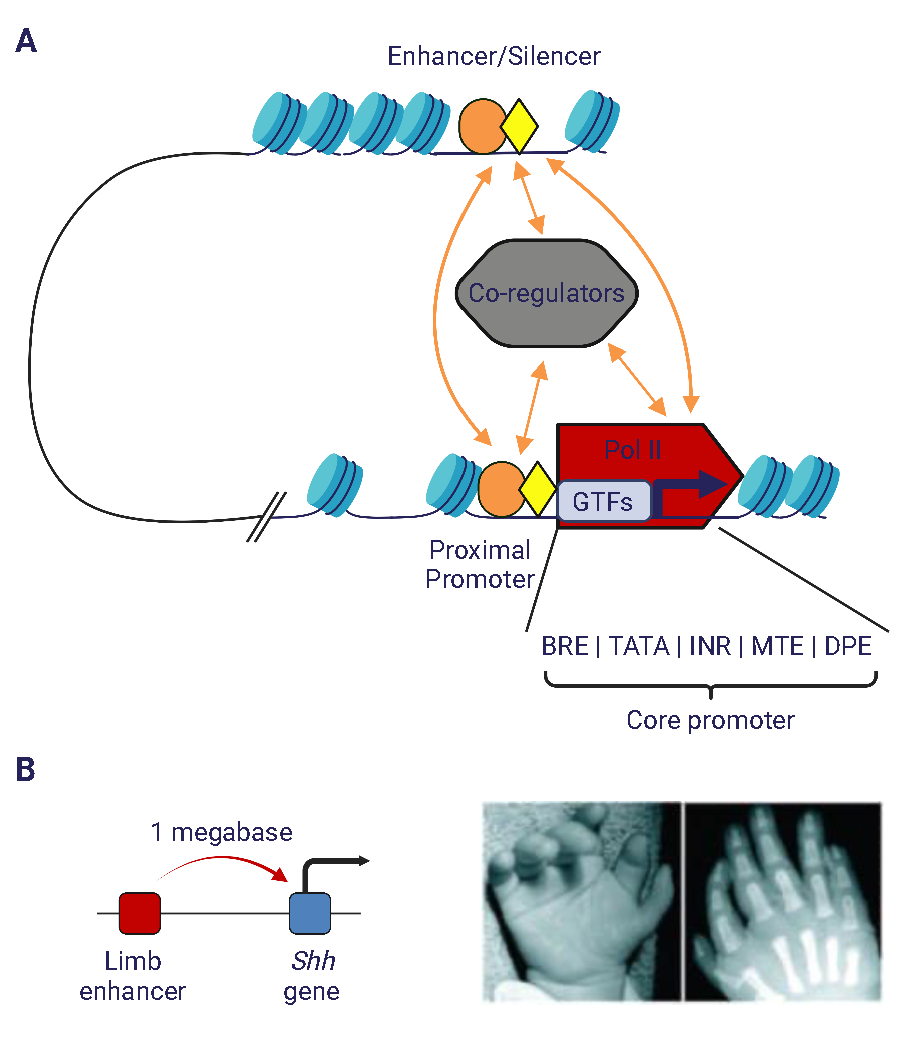
\includegraphics[width=0.8\textwidth]{chapter1/figures/fig1.pdf}
    \caption[\textit{Cis}-regulatory elements in the genome]{\textbf{\textit{Cis}-regulatory elements in the genome. (A)} Schematic view of \textit{cis}-regulatory elements around the core promoter, proximal promoter and enhancer/silencer regions. The \textit{cis}-regulatory elements within the core promoter including BRE, TATA, INR, MTE and DPE elements are bound by the general transcription factors (GTFs, blue rectangle). Other responsive elements within the proximal promoter and enhancer/silencer regions are recognised by regulatory transcription factors (orange ovals and yellow diamonds). Co-regulators (grey hexagon) are indirectly associated with the \textit{cis}-regulatory elements by binding to the transcription factors. Transcription factors and co-regulators regulate the transcription mediated by the RNA polymerase II (Pol II, red rocket). Orange and black arrows indicate the protein-protein interaction and the transcription start site respectively. \textbf{(B) Left,} schematic view of the spatial-relationship between the limb enhancer and the \textit{Shh} gene. \textbf{Right,} an example of hands from the patient with a single point mutation in the \textit{Shh} gene limb enhancer region (adapted from \cite{fuda2009defining} and \cite{visel2009genomic}).}
    \label{fig:fig1}
\end{figure}

The genetic code is stored in the coding exons within the gene body, but the information that controls the spatial-temporal expression of a gene is encoded in the DNA sequences called \textit{cis}-regulatory elements. In general, the DNA sequences within these regions can target the assembly of transcription factor complexes, consequently activating or repressing the transcription of a gene. The \textit{cis}-regulatory element can be mainly categorised into three groups according to its distance relative to the transcription start site (TSS) of a gene: the core promoter, the proximal promoter, and the enhancer/silencer (reviewed in \cite{visel2009genomic}). The core promoter is mostly located within tens of base pairs of a TSS. Common core promoter elements include the TATA box (TATA), the TFII\underline{B} \underline{r}ecognition \underline{e}lement (BRE), the \underline{in}itiato\underline{r} element (INR), the \underline{m}otif \underline{t}en \underline{e}lement (MTE), and the \underline{d}ownstream \underline{p}romoter \underline{e}lement (DPE). These elements can be bound by the general transcription factors which help recruit the \underline{p}re-\underline{i}nitiation \underline{c}omplex (PIC) and subsequently specify the TSS (reviewed in \cite{juven-gershon2008the}). The proximal promoter is close, usually upstream, to the core promoter, and the enhancers/silencers are generally located at distal regions from the TSS. The promoter and enhancer/silencer contain DNA sequences called \underline{r}esponsive \underline{e}lements (REs) which can be recognised by sequence-specific binding transcription factors. They help recruit transcription activators/repressors and consequently change the transcription of the downstream genes (\textbf{Figure \ref{fig:fig1}A})(reviewed in \cite{fuda2009defining}).

Besides the recruitment of transcription factors by pure DNA sequences, the nucleotides within the \textit{cis}-regulatory element also undergo modifications which often affect gene transcription. For example, the cytosines in the CpG sites in mammals tend to be methylated to 5-methylcytosine (5mC) which is usually associated with mutation (5mc $\rightarrow$ T) and gene silencing (reviewed in \cite{deaton2011cpg}). In addition, recent studies have shown that enzymes from the Tet family can catalyse the conversion of 5mC to 5hmC which is prevalent in mammalian cells, especially in neuronal cells of the central nervous system (\cite{kriaucionis2009the,tahiliani2009conversion}).

Though they do not directly encode proteins, the \textit{cis}-regulatory elements are equally important as the protein-coding sequences. This can be demonstrated by the discovery that a single nucleotide mutation within the limb enhancer, which is located at 1 megabase away from the \textit{Shh} gene and does not encode any proteins, severely disturbs the proper limb formation in mouse and human (\textbf{Figure \ref{fig:fig1}B}) (\cite{lettice2003a,sagai2005elimination}). Recent genomic studies strongly suggest variations in \textit{cis}-regulatory elements in gene expression (reviewed in \cite{visel2009genomic}).

\subsection{Transcription factors} \label{section:tf}

Transcription factors can decipher the code held within the \textit{cis}-regulatory element by directly binding to their responsive elements to regulate gene transcription. Generally, transcription factors can be divided into two distinct groups (\cite{lemon2000orchestrated}):

\textbf{(1) General transcription factors (GTFs):} \underline{G}eneral \underline{t}ranscription \underline{f}actors (GTFs) include TFIIA, TFIIB, TFIID, TFIIE, TFIIF, and TFIIH (reviewed in \cite{reese2003basal,thomas2006the,sikorski2009the}). Together with Pol II, GTFs bind to the aforementioned cis-regulatory elements within the core promoter regions to form the PIC, which is a significant event in transcription initiation (reviewed in \cite{juven-gershon2008the}).

\textbf{(2) Regulatory transcription factors:} Regulatory transcription factors can recognise and bind to specific DNA sequences, \textit{i.e.} their responsive elements, within the proximal promoter or enhancer/silencer regions by their \underline{D}NA-\underline{b}inding \underline{d}omain (DBD) to either activate (activators) or repress (repressors) transcription. These factors usually facilitate the formation and the stabilisation of the PIC, or help the recruitment of required co-regulators and chromatin-modifying factors, which results in a change of the gene transcription (reviewed in \cite{ptashne1988how,narlikar2002cooperation}). In this study and most research papers, the term \enquote{transcription factor} generally refers to this kind of transcription factors. Usually, transcription factors are classified according to their DBDs. Among them are the well-known domains: helix-turn-helix (\textit{e.g.}, homeobox), helix-loop-helix (\textit{e.g.}, MyoD and Myogenin), zinc finger (\textit{e.g.}, SP1), basic leucine zipper (\textit{e.g.}, c-Jun and c-Fos) (reviewed in \cite{latchman1997transcription}).

In addition to DNA-binding transcription factors, other proteins like co-regulators and chromatin-modifying factors which do not directly contact DNA are also important for the transcriptional regulation of a gene. Co-regulators generally provide additional connections between regulatory transcription factors and the GTFs or Pol II through protein-protein interactions, leading to the activation or repression of the gene (reviewed in \cite{näär2001transcriptional}).

Chromatin-modifying factors contain two kinds of complex: (1) chromatin remodellers, enzymes that reposition, reconfigure or eject nucleosomes in a noncovalent manner using the energy from ATP hydrolysis (reviewed in \cite{cairns2009the,becker2002atp-dependent}), and (2) chromatin modifiers, enzymes that covalently modify nucleosomes (\cite{cairns2009the,narlikar2002cooperation}).

Chromatin remodellers are able to disrupt the interaction between the DNA and the core histone surface, which results in either a displacement or a shift of histone octamers to adjacent positions (reviewed in \cite{narlikar2002cooperation}). Chromatin modifiers covalently change nucleosomes by modifications of histone tails such as acetylation, methylation, phosphorylation, ubiquitination, and sumoylation (reviewed in \cite{narlikar2002cooperation,bannister2005reversing,shilatifard2006chromatin}). These modifications not only alter the electrostatic DNA-histone interaction, but also provide docking sites for the recruitment of non-histone regulatory proteins and the transcription machinery, subsequently leading to transcription activation or repression.

\subsection{Transcription stages}

Transcription is a multistage process, which consists of at least six major steps (\textbf{Figure \ref{fig:fig2}}): chromatin remodelling, initiation, Pol II pausing, elongation, termination, and re-initiation (reviewed in \cite{fuda2009defining}).

\begin{figure}[!ht]
    \centering
    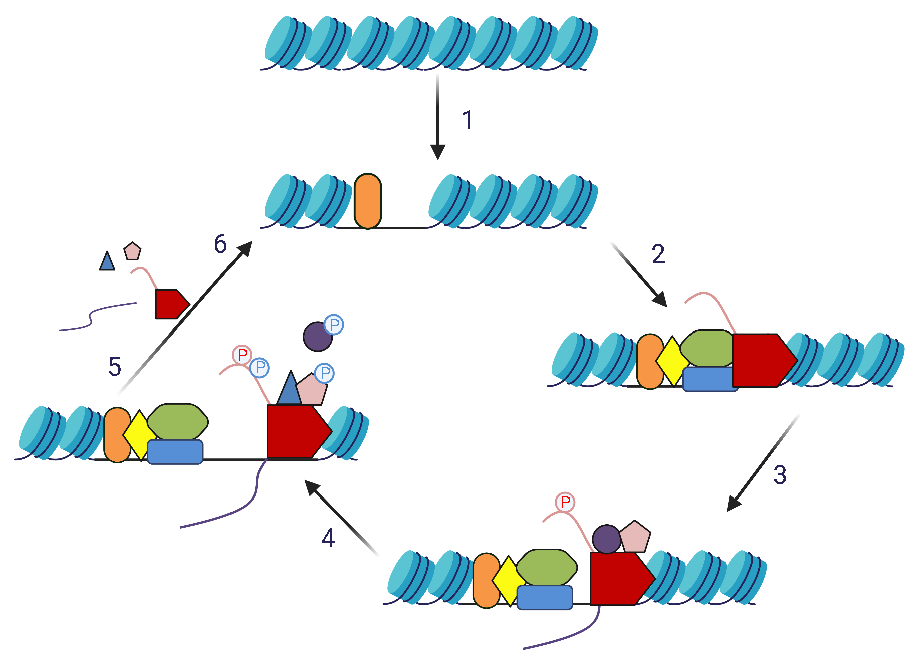
\includegraphics[width=0.9\textwidth]{chapter1/figures/fig2.pdf}
    \caption[Different stages of transcription]{\textbf{Different stages of transcription. Stage 1:} chromatin remodelling. The gene and its regulatory regions are packaged as nucleosomes (light brown). An activator (orange ovals) binds to DNA and recruits chromatin remodelling complex to make the promoter open for transcription factor binding. \textbf{Stage 2:} initiation. A second activator (yellow diamond) binds, promotes the binding of GTFs (blue rectangles) and recruits co-activators (green hexagons), facilitating Pol II (red rocket) entry to the PIC. Consequently, DNA is unwound at the TSS, and an open complex is formed. \textbf{Stage 3:} Pol II pausing. Pol II breaks contacts with promoter-bound factors, transcribes 20 - 50 bases downstream of the TSS, produces an RNA (purple lines) and pauses, which is mediated by DSIF (pink pentagon) and NELF complex (purple circle). The Ser residues at position 5 (Ser 5) of the Pol II carboxyl-terminal domain (CTD) repeats are phosphorylated (red Ps) during this stage. \textbf{Stage 4:} elongation. P-TEFb (blue triangles) is recruited directly or indirectly by the activator and phosphorylates Ser 2 of the Pol II CTD repeats, DSIF and the NELF subunits (blue Ps). NELF dissociates from the rest of the complex. Pol II escapes from the pause, travelling along the gene body. Productive elongation happens. \textbf{Stage 5:} termination. After the Pol II complex transcribes the gene, it is removed from the DNA, and the RNA is released. \textbf{Stage 6:} re-initiation. The freed Pol II can re-initiate (adapted from \cite{fuda2009defining})}
    \label{fig:fig2}
\end{figure}

\subsubsection{Stage 1: Chromatin remodelling}

In eukaryotes, the DNA is wrapped around histone octamers to form nucleosomes, the fundamental units of eukaryotic chromatin (\cite{kornberg1974chromatin}). Although this kind of DNA wrapping compacts the genome, it also prevents transcription initiation by restricting the DNA-binding events of transcription factors (reviewed in \cite{cairns2009the}). Therefore, the occurrence of transcription requires changes of chromatin structure by chromatin- modifying factors, so that transcription factors and Pol II can gain access to the promoter of a gene (\cite{boeger2003nucleosomes}).

\subsubsection{Stage 2: Transcription initiation}

The second stage of transcription is initiation, the most extensively-studied event during the process of transcription. Transcription initiation begins with the formation of PIC (reviewed in \cite{martinez2002multi-protein}). At the start of PIC formation, TFIID binds to the core promoter elements, followed by TFIIB binding to the promoter. Together, they recruit other GTFs and Pol II through either a sequential assembly or a preassembled Pol II holoenzyme pathway (reviewed in \cite{thomas2006the}). \textit{In vitro} studies show that the PIC is sufficient for basal levels of transcription (\cite{reese2003basal,thomas2006the}). However, this complex does not respond to activators and cannot start transcription of chromatin templates \textit{in vivo} (reviewed in \cite{sikorski2009the}). Therefore, a multitude of co-regulators and chromatin-modifying factors are also needed in the promoter region of the gene. For example, Mediators can bind to the carboxyl terminal domain (CTD) of Pol II, connecting Pol II and other transcription factors, which is required for most Pol II mediated transcription (reviewed in \cite{björklund2005the}). The regulatory transcription factors, the co-regulators, the chromatin-modifying factors, together with the PIC and gene promoters, are connected with each other, forming a transcription initiation complex through protein-protein and protein-DNA interactions. After formation of this initiation complex, transcription will enter into the next stage.

\subsubsection{Stages 3-6: Pol II pausing, elongation, termination, and re-initiation}

It was once believed that transcription was rarely regulated during the stages after the initiation. However, some early studies at the gene-specific level demonstrated that certain genes, such as the \textit{Drosophila Hsp70} gene, experience transcription initiation but show no productive elongation, \textit{i.e.} the Pol II is paused at the promoter regions (\cite{rougvie1988the}). This is the first clue of the existence of post-initiation regulatory stages. Recent genome-wide studies suggest the Pol II pausing is prevalent and important for metazoan protein-coding genes, especially those that are involved in stimulus-responsive gene networks (\cite{guenther2007a,gilchrist2012regulating}). After the transcription initiation, the pausing factors \underline{ne}gative \underline{el}ongation \underline{f}actor (NELF) and \underline{D}RB-\underline{s}ensitivity \underline{i}nducing \underline{f}actor (DSIF) generate a paused Pol II just downstream of the TSS (\cite{yamagata2008arginine}). The release of the paused Pol II to productive elongation requires the recruitment of the \underline{p}ositive \underline{t}ranscription \underline{e}longation \underline{f}actor \underline{b} (P-TEFb) to the paused Pol II, which subsequently phosphorylates the components in the initiation complex, including Pol II, NELF, and DSIF (\cite{core2008transcription}). A more recent study shows that the transcription factor c-Myc recruits P-TEFb to help the escape of paused Pol II (\cite{rahl2010c-myc}). Once escaped from the pausing, productive elongation will occur. Transcription termination and re-initiation are the least characterised stages.

In this study, we only concentrate on the first two stages of transcription: chromatin remodelling and initiation.

\section{The cell cycle regulation}

\subsection{General characteristics of the cell cycle events}

The cell cycle is the sequence of highly regulated processes during which cells make exact replicas of themselves. The smooth progression of the cell cycle requires cyclic expressions of certain genes: they must be activated and only be activated at specific phases. Failure of activation or repression at the proper time often results in abnormal cell cycle events. The series of highly dynamic events during the cell cycle provide a perfect model for the study of the transcriptional regulation. In addition, since the cell cycle is a very basic and prevalent biological process, many cell cycle regulators and events are evolutionarily conserved.

The eukaryotic cell cycle is conventionally divided into four distinct phases: the DNA synthesis phase (S phase), the segregation of duplicated chromosomes during mitosis (M phase), and two gaps, one before (G1 phase) and one after (G2 phase) S phase (\textbf{Figure \ref{fig:fig3}A}). When cells are exposed to extracellular conditions that arrest cell proliferation, such as serum starvation which is a common method in laboratories to synchronise cells, they can leave the cell cycle and enter a quiescent state termed G0 phase, where they can remain for days, weeks or even years before re-entering the cell cycle (reviewed in \cite{62}).

\begin{figure}[!ht]
    \centering
    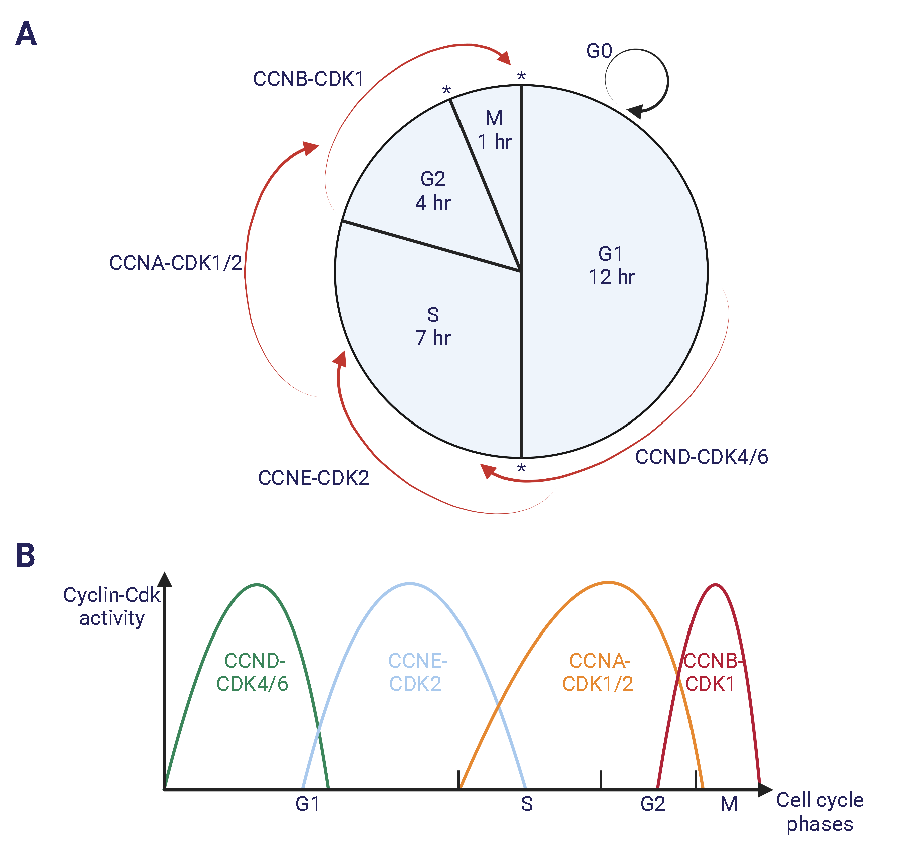
\includegraphics[width=0.8\textwidth]{chapter1/figures/fig3.pdf}
    \caption[The classical and minimal models of the cell-cycle control]{\textbf{The classical and minimal models of the cell-cycle control. (A)} Schematic view of the regulation of cell cycle progression by the relay of different Cyclin-Cdk complexes. Checkpoints (*) and the duration of each phase of a typical mammalian cell cycle are indicated. \textbf{(B)} Simplified view of activities of various Cyclin-Cdk complexes at different phases of the cell cycle (adapted from \cite{hochegger2008cyclin-dependent}).}
    \label{fig:fig3}
\end{figure}

The progression of the cell cycle requires at least three transitions, also called checkpoints, at the onset of S phase and at entry and exit of mitosis. All key stages in the cell cycle are subjected to these transitions, at which cells will \enquote{check} whether earlier processes, such as DNA replication and chromosome segregation, have been properly completed. Cells have the option to arrest the cell cycle if something goes wrong, preventing \enquote{abnormal} cells from proceeding to the next stage. At the heart of these switch-like transitions are the \underline{c}yclin-\underline{d}ependent \underline{k}inases (CDKs) and their regulatory subunits termed cyclins (reviewed in \cite{nurse2000a,hochegger2008cyclin-dependent}).

The CDKs, which have been described as a \enquote{cell cycle engine}, are serine/threonine protein kinases that drive cells through the cell cycle (reviewed in \cite{ds}). They are generally inactive without their cyclin partners. In most cases, the levels of CDKs are relatively constant throughout the cell cycle, whereas the concentration of most cyclins oscillates. Each CDK is activated by binding to its relevant cyclin during specific phases of the cell cycle, and in turn promotes phosphorylation of target substrates required for cell cycle progression. Therefore, progression through the various phases of the cell cycle is coordinated by waves of activation of CDKs. According to the traditional view once the cell enters into G1 phase after receiving appropriate signals, cyclin D (CCND)- CDK4/6 complexes are required during the progression of G1; at the G1/S checkpoint, CCNE-CDK2 complex is needed to start S phase; then CCNA-CDK1/2 complexes are responsible for the execution of S phase; at G2/M checkpoint, the CCNB-CDK1 complex is indispensable for the entry and progression of mitosis (\textbf{Figure \ref{fig:fig3}B}). However, this model has been challenged by recent studies indicating that mice that lack CDK2 are viable and healthy (\cite{ortega2003cyclin-dependent,berthet2003cdk2}). A more recent study uses mouse embryos lacking all CDKs that are thought to be essential in interphase (CDK2, CDK3, CDK4 and CDK6) and reveals that CDK1 is sufficient to drive all the events during the cell cycle. In this situation, CDK1 bound to all cyclins, leading to the proceeding of cellular events, such as phosphorylation of retinoblastoma protein pRb, which is required for S phase entry (\cite{santamaría2007cdk1}). Studies of \textit{Cdk} knock-out mice have shown us that deletion of \textit{Cdk1} is lethal (\cite{santamaría2007cdk1}). In addition, deletion of other \textit{Cdks} in mice results in some functional deficiencies, such as sterility (\textit{Cdk2}) (\cite{ortega2003cyclin-dependent,berthet2003cdk2}) and lack of adult pancreatic $\beta$-cells and pituitary lactotrophs (\textit{Cdk4}) (\cite{rane1999loss}), but these mice are viable and even healthy. These studies inform us that only CDK1 is essential for the cell survival, while other CDKs are also needed to maintain normal functions of the cell. It has become clear that there are many other complex events driving the cell cycle, besides the sequential activation of various CDKs.

\subsection{Transcriptional regulation of mammalian G2-M genes}

As mentioned above, the cyclic expression of cell cycle genes is critical for the smooth progression of the cell cycle. Genes that are required for G2 and M progression must be kept inactive during G0 or G1 phase and turned on at the proper time during G2 and M phase. In mammals, this temporal expression is controlled by the DNA elements called the CDE (\underline{c}ell cycle-\underline{d}ependent \underline{e}lement) and the CHR (\underline{c}ell cycle genes \underline{h}omology \underline{r}egion) within their promoters. In addition, the CCAAT-box element which is bound by the transcription factor NF-Y is also present in most cell cycle genes, though not restricted to G2-M genes, and is required for the activation of the gene (reviewed in \cite{müller2010the}). The CDE is a 6 base pair long GC-rich sequence, and a typical CHR consensus is TTTRAA where R represents an A or G (reviewed in \cite{müller2010the}). Early studies suggest that the CDE and the CHR elements are important for keeping the G2-M genes repressed during G0 and G1 phases, as mutations of these two elements in quiescent cells result in the hyperactivation of G2-M genes in resting cells (\cite{lucibello1995periodic,tommasi1995in,zwicker1995cell}). A most recent study demonstrates that the CHR element is absolutely required for both the repression and the activation of the G2-M genes, but the CDE element is not always present in the promoters (\cite{müller2012the}). Mutation of the CDE element has marginal effects on gene expression in most cases, but disruption of the CHR element unanimously gives rise to deregulation of the G2-M genes, leading to a derepression during G0 and a failure of activation in G2 and M phases (\cite{müller2012the}). Indeed, sequence alignment across different species of promoters from typical genes whose expression peak at the G2 and M phases shows that only the CHR and the CCAAT-box, not the CDE element, is evolutionarily conserved (\textbf{Figure \ref{fig:fig4}A}) (reviewed in \cite{müller2010the}).

A lot of CDE/CHR containing genes are negatively regulated by the tumour suppressor p53 (reviewed in \cite{müller2010the}). In many cases, the p53-dependent repression is, in part, through the CDE/CHR elements, though these elements are not directly bound by p53 (reviewed in \cite{müller2010the}). Only recently has an evolutionarily conserved multi-subunit protein complex been revealed to regulate the cell cycle gene expression through the CHR element. In G0 phase, the transcription factors DP and E2F4, together with RBL2 (a.k.a p130) and homologs of the \textit{C. elegans} synthetic \underline{mu}lti\underline{v}ulva class \underline{B} (MuvB) including LIN9, LIN37, LIN52, LIN54, and LIN53/RBBP4, are associated together to form a complex, namely DREAM, sitting on the promoters of most cell cycle genes to keep them repressed. When cells enter the cell cycle, the DREAM complex dissociates from the promoters of the cell cycle genes, resulting in the loss of repression of the genes that are required for the cell cycle. In the meantime, MuvB is separated from DP, E2F4 and RBL2 and interacts with another transcription factor B-MYB (a.k.a MYBL2), forming a new complex called MMB. In G2 and M phases, the MMB complex binds to the promoters of many genes that are required for the G2-M transition (but not genes that are required for G1-S transition) to activate their expression (\cite{litovchick2007evolutionarily,müller2012the,sadasivam2012the}). Importantly, the binding of the DREAM/MMB complexes to the DNA requires an intact CHR element in the promoter of the G2-M gene (\cite{müller2012the}) (\textbf{Figure \ref{fig:fig4}B}).

\begin{figure}[!t]
    \centering
    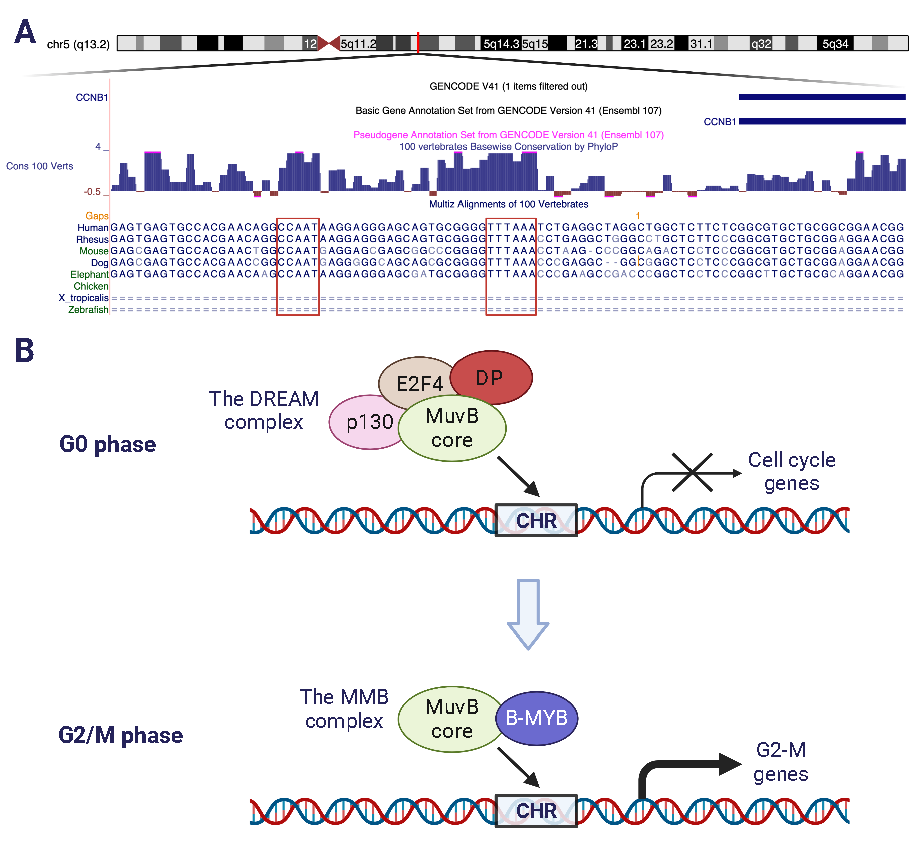
\includegraphics[width=0.8\textwidth]{chapter1/figures/fig4.pdf}
    \caption[The CHR element and the DREAM/MMB complex are important for the regulation of G2-M transition]{\textbf{The CHR element and the DREAM/MMB complex are important for the regulation of G2-M transition. (A)} Sequence alignment of the promoter of \textit{CCNB1}, a typical gene that is required for the G2-M transition, across different species. Two highly conserved elements the CCAAT-box and the CHR motifs are highlighted. \textbf{(B)} Schematic and simplified view of the regulation of the cell cycle by the DREAM/MMB complexes. In G0 phase, the MuvB core interacts with E2F4, DP1, and p130 (the DREAM complex) to keep the cell cycle genes repressed. This repression is mediated by the CHR motif. When cells enter the cell cycle, the DREAM complex dissociates from the promoters and disassembles, resulting in derepression of the cell cycle genes. In G2 and M phases, the MuvB core comes back to the promoter of genes that are required for G2-M transition (but not for G1-S transition) together with B-MYB (the MMB complex), leading to the activation of the genes. The activation is also mediated through the CHR motif.}
    \label{fig:fig4}
\end{figure}

Interestingly, the DREAM-like complex is also observed in flies and worms, though there are some differences in the components (\cite{Beall2002-mq,korenjak2004native}). Due to the lack of a B-MYB ortholog in worms, the MMB-like complex is only seen in mammals and flies (\cite{harrison2006some}). The roles of the CHR element and the DREAM/MMB complexes in cell cycle regulation were discovered separately, and have finally converged recently.

\section{Forkhead transcription factors}

\subsection{General characteristics of Forkhead transcription factors}

The defining feature of Forkhead transcription factors is the evolutionarily conserved DNA-binding domain: the Forkhead box (FOX) domain, which contains approximately 110 amino acid residues. The first discovered member of Forkhead transcription factor family was the region-specific homeotic gene \textit{forkh head (fkh)}. Mutation of this gene caused spiked-head structures in embryos of the \textit{Drosophila}, hence the name fork head (\cite{weigel1989the}). Over 100 genes encoding Forkhead proteins were later detected in various species ranging from yeast to human (reviewed in \cite{lai1993hepatocyte,kaufmann1996five}). X-ray crystallographic analysis and NMR spectroscopic analysis have shown that the canonical Forkhead box resembles a \enquote{winged helix} structure, which contains three $\alpha$-helices, three $\beta$-sheets and two loops or wings, typically arranged in an order of \enquote{$\alpha 1 - \beta 1 - \alpha 2 - \alpha 3 - \beta 2 - W1 - \beta 3 - W2 $} (see \textbf{Chapter \ref{ch:discussion}, Figure \ref{fig:fig53}}) (\cite{clark1993co-crystal,jin1999dynamic,van-dongen2000solution}). The primary binding interaction is through the third $\alpha$-helix ($\alpha 3$) which makes direct contacts with the target DNA in the major groove (\cite{clark1993co-crystal,marsden1998structural}).

It has been 20 years since the discovery of the first member of Forkhead transcription factor family. Hundreds of Fox genes have been identified from various species, and the number of Fox genes seems to rise with the increase of their anatomical complexity, from four in budding yeast to over forty in humans (reviewed in \cite{wijchers2006in,hannenhalli2009the}).

\subsection{Forkhead transcription factors and the cell cycle}

Forkhead (FOX) transcription factors are indispensable in regulating the expression of genes that are essential in a diverse range of biological processes, from cell cycle control to stress resistance, from language acquisition to appetite and body weight control. A subset of FOX proteins are key players in the cell cycle control, which have attracted a lot of attention.

\subsubsection{Fkh2p and the cell cycle control in budding yeast}

In yeast, the \textit{CLB2} gene cluster whose transcription level peaks at the G2 and M phase contains 33 genes, such as \textit{CLB1}, \textit{CLB2}, \textit{SWI5}, \textit{CDC5}, \textit{CDC20} and other genes which are critical for the events during mitosis (\cite{spellman1998comprehensive}). The transcription of genes within this cluster is controlled by a transcription factor complex that consists of the MADS-box transcription factor Mcm1p, the Forkhead transcription factor Fkh2p, and the coactivator Ndd1p (\cite{koranda2000forkhead-like,darieva2006polo}) (\textbf{Figure \ref{fig:fig5}}, top panel). The activity of this ternary complex is regulated through sequential phosphorylation of Fkh2p by the cyclin-cdk complex Clb5p-Cdc28p (\cite{pic-taylor2004regulation}), and Ndd1p by Clb2p- Cdc28p (\cite{darieva2003cell,reynolds2003recruitment}) and by Cdc5p (\cite{darieva2006polo}). Interestingly, Clb2p and Cdc5p themselves are also encoded by the genes within the \textit{CLB2}  cluster. Hence, this mode of transcription generates a positive feedback loop during the G2 and M phases, ensuring the smooth progression of the cell cycle at these stages (\textbf{Figure \ref{fig:fig5}}, top panel).

\subsubsection{FOXM1 and the cell cycle control}

Mammalian FOXM1 is a proliferation-specific transcription factor which exhibits cell cycle-dependent expression. Both FOXM1 mRNA and protein levels are barely detectable in quiescent cells and are at relatively low levels in G1 phase. The expression (both mRNA and protein) of FOXM1 begins to increase in S phase, peaks when cells enter G2 and M phases, and then decreases at the late M phase (\cite{ye1997hepatocyte,korver1998uncoupling,park2008anaphase-promoting}). There are three isoforms of human FOXM1 protein due to differential splicing of two alternative exons: FOXM1a, FOXM1b and FOXM1c. Both FOXM1b and FOXM1c are transcription activators, whereas FOXM1a does not transactivate because of an additional exon in the C-terminal transactivation domain (reviewed in \cite{laoukili2007foxm1:}). Until now, only FOXM1b and FOXM1c have been studied, which together are referred to as FOXM1 in the following section unless otherwise specified.

\begin{figure}[!t]
\centering
    \begin{tikzpicture}
        \draw (0,3.5) node[anchor=west] {\small \textbf{Budding yeast}};
        \draw (11,0) node[draw, very thick, anchor=south, fill=pink!60] {\small \textbf{Cdc5p}};
        \draw (11,0.75) node[draw, very thick, anchor=south, fill=red!60] {\small \textbf{Clb2p}};
        \draw[ultra thick] (3.5,1.5) -- (10,1.5);
        \draw[ultra thick, ->, >={Triangle[scale=0.5]}] (9,1.5) -- (9,2.25) (9,2.25) -- (11,2.25) node[anchor=south, pos=0.5] {\small \textit{CLB2} cluster};
        \draw (7,5.5) node[draw, very thick, anchor=south, fill=pink!60] {\small \textbf{Cdc5p}}
              (3.5,5.5) node[draw, very thick, fill=blue!60] {\small \textbf{Cdc28p}}
              (4,5) node[draw, very thick, fill=red!60] {\small \textbf{Clb2p}};
        \draw[very thick, fill=cyan] (7,2) circle[x radius=1, y radius=0.5];
        \draw[very thick, fill=green!70] (5.75,2.75) circle[x radius=1, y radius=0.5];
        \draw[very thick, fill=yellow!75] (5,2) circle[x radius=1, y radius=0.5];
        \draw[draw=none, fill=magenta, opacity=0.9] (4.25,2.4) circle[radius=0.2]
             (5,3.15) circle[radius=0.2] (6.5,3.15) circle[radius=0.2];
        \draw (7,2) node {\small \textbf{Mcm1p}} (5,2) node {\small \textbf{Fkh2p}} (5.75,2.75) node {\small \textbf{Ndd1p}} (4.25,2.4) node (p1) {\scriptsize P} (5,3.15) node (p2) {\scriptsize P} (6.5,3.15) node (p3) {\scriptsize P};
        \draw[->, very thick, >={Triangle[scale=0.5]}] (4,4.5) -- (p1.north);
        \draw[->, very thick, >={Triangle[scale=0.5]}] (4.25,4.5) -- (p2.north);
        \draw[->, very thick, >={Triangle[scale=0.5]}] (7,5.25) -- (p3.north);
        \draw[->, very thick, >={Triangle[scale=0.5]}] (12,0.75) -- (13,0.75) (13,0.75) -- (13,5.5) (13,5.5) -- (8,5.5);
    \end{tikzpicture}
    \begin{tikzpicture}
        \draw (0,3.5) node[anchor=west] {\small \textbf{Mammal}};
        \draw (11,0) node[draw, very thick, anchor=south, fill=pink!60] {\small \textbf{PLK1}};
        \draw (11,0.75) node[draw, very thick, anchor=south, fill=red!60] {\small \textbf{CCNB}};
        \draw[ultra thick] (3.5,1.5) -- (10,1.5);
        \draw[ultra thick, ->, >={Triangle[scale=0.5]}] (9,1.5) -- (9,2.25) (9,2.25) -- (11,2.25) node[anchor=south, pos=0.5] {\small \textit{G2/M} genes};
        \draw (7,5.5) node[draw, very thick, anchor=south, fill=pink!60] {\small \textbf{PLK1}}
              (3.5,5.5) node[draw, very thick, fill=blue!60] {\small \textbf{CDK1}}
              (4,5) node[draw, very thick, fill=red!60] {\small \textbf{CCNB}};
        \draw[very thick, fill=cyan] (3.25,2.25) circle[x radius=0.75, y radius=0.375];
        \draw[very thick, fill=green!70] (3.25,3.25) circle[x radius=0.75, y radius=0.375];
        \draw[very thick, fill=yellow!75] (6.25,2) circle[x radius=1, y radius=0.5];
        \draw[draw=none, fill=magenta, opacity=0.9] (5.5,2.4) circle[radius=0.2]
             (6.25,2.5) circle[radius=0.2] (7,2.4) circle[radius=0.2];
        \draw (3.25,2.25) node {\small \textbf{SRF}} (6.25,2) node {\small \textbf{FOXM1}} (3.25,3.25) node {\small $\times$} (5.5,2.4) node (p1) {\scriptsize P} (6.25,2.5) node (p2) {\scriptsize P} (7,2.4) node (p3) {\scriptsize P};
        \draw[->, very thick, >={Triangle[scale=0.5]}] (4,4.5) -- (p1.north);
        \draw[->, very thick, >={Triangle[scale=0.5]}] (4.25,4.5) -- (p2.north);
        \draw[->, very thick, >={Triangle[scale=0.5]}] (7,5.25) -- (p3.north);
        \draw[->, very thick, >={Triangle[scale=0.5]}] (12,0.75) -- (13,0.75) (13,0.75) -- (13,5.5) (13,5.5) -- (8,5.5);
    \end{tikzpicture}
    \caption[Transcription programs that regulate the G2-M transition of yeast and human cell cycles]{\textbf{Transcription programs that regulate the G2-M transition of yeast and human cell cycles. Top,} schematic view of the positive feedback loop between the Mcm1p-Fkh2p-Ndd1p ternary complex and the proteins encoded by the CLB2 cluster in budding yeast. \textbf{Bottom,} schematic view of the positive feedback loop between FOXM1 and proteins that are required for the mitosis in mammals. The homologous proteins are drawn in matching colours, and the phosphorylation events are indicated by black arrows and pink Ps.}
    \label{fig:fig5}
\end{figure}

Many recent studies point out that FOXM1 is a master regulator of the G2 and M phase progression of the cell cycle. Knockdown of FOXM1 causes polyploidy and a delay in G2 (\cite{laoukili2005foxm1}). Both the depletion and the overexpression of FOXM1 induce the deregulation of a large array of genes that are required for the G2 phase and mitosis, and the yeast homologs of many FOXM1 target genes are within the \textit{CLB2} cluster (\cite{laoukili2005foxm1,wonsey2005loss,lefebvre2010a}). Like the ternary complex Mcm1p-Fkh2p-Ndd1p, the transcriptional activity of FOXM1 is also regulated by sequential phosphorylation by Cyclin-Cdk kinase complexes CCNA-CDK1/2, CCNB- CDK1 and by PLK1 (\cite{wang2005forkhead,fu2008plk1-dependent,laoukili2008activation}). Very intriguingly, CDK1, CCNB, and PLK1 are the mammalian orthologs of yeast Cdc28p, Clb2/5p, and Cdc5p respectively. Furthermore, \textit{CDK1}, \textit{CCNB}, and \textit{PLK1} are also FOXM1 target genes (\cite{laoukili2005foxm1,wang2005forkhead}). Clearly, a similar positive feedback loop also exists in mammalian cells to secure the progression of the G2 phase and mitosis (\textbf{Figure \ref{fig:fig5}}, bottom panel), although some differences are apparent: no evidence so far suggests that SRF, the mammalian MADS-box transcription factor, interacts with FOXM1 or the promoters of genes expressed in late G2 and M phases, and there is no Ndd1p ortholog in mammals or any other organisms (reviewed in \cite{murakami2010regulation}). It seems that FOXM1 is comparatively similar to the yeast Fkh2p, though they do not share any apparent homology at regions outside the Forkhead domain.

The positive feedback loop during the G2 phase and mitosis, mediated by Mcm1p- Fkh2p-Ndd1p in yeasts, and by FOXM1 in mammals, emphasises the importance of the Forkhead transcription factors in cell cycle control. In addition, the conservation of the components within the positive feedback loop also provides a good model for evolutionary studies.

\subsubsection{FOXOs and cell cycle control}

Another important set of regulators in the cell cycle control are the FOXO subfamily of Forkhead transcription factors, which share high sequence homology to the \textit{Caenorhabditis elegans} Forkhead transcription factor DAF-16 (reviewed in \cite{myatt2007the}). Actually, one of the first functions discovered for FOXOs was that they could regulate the G1/S transition (\cite{medema2000afx-like}). Currently, four FOXO isoforms have been identified in mammalian cells: FOXO1, FOXO3, FOXO4 and FOXO6. The expression of \textit{FOXO6} is limited to brain, thymus and kidney, whereas \textit{FOXO1}, \textit{FOXO3} and \textit{FOXO4} are ubiquitously expressed (reviewed in \cite{greer2005foxo}). Of note, in mammals, there are two \textit{FOXO3} genes, \textit{FOXO3a} and \textit{FOXO3b}, but \textit{FOXO3b} turns out to be a pseudogene (\cite{greer2005foxo}). The terms \textit{FOXO3A} and \textit{FKHRL1} are the most commonly-used names for the \textit{FOXO3} gene, but according to the HGNC (HUGO Gene Nomenclature Committee), the latest official gene symbol of this gene is \enquote{FOXO3} (\url{https://www.genenames.org/data/hgnc_data.php?hgnc_id=3821}). Therefore, \enquote{FOXO3} is used in this study. FOXO proteins have long been shown to play important roles in cell cycle arrest. Like other transcription factors, the transcriptional activities of FOXOs are extensively regulated by post-translational modifications like phosphorylation, methylation and acetylation (\cite{brunet1999akt,matsuzaki2005acetylation,yamagata2008arginine}). Phosphorylation is the most extensively-studied modification of the FOXO proteins.

Unlike Fkh2p and FOXM1, the phosphorylation of FOXOs mostly results in the inhibition of their transcriptional activities (\cite{brunet1999akt}). The FOXO proteins are key direct targets of the phosphatidylinositol 3-kinase (PI3K)-AKT signalling pathway (\cite{brunet1999akt}). AKT phosphorylates FOXOs at three important regulatory sites (Thr32, Ser253, and Ser315 in FOXO3 protein) which are conserved from worms to mammals (reviewed in \cite{greer2005foxo}). This AKT-mediated phosphorylation induces the nuclear export of FOXOs by the 14-3-3 proteins, which serve as chaperone molecules to escort them out of the nucleus, leading to the loss of transcriptional activity of FOXOs (\cite{brunet1999akt,brunet200214-3-3}). Similarly to the positive feedback loop in promoting the G2 and M phase progression, this PI3K-AKT-FOXO signalling cascade is also evolutionarily conserved from worms to mammals (\textbf{Figure \ref{fig:fig6}}).

The importance of this PI3K-AKT-FOXO signalling is underlined by the highly activated PI3K-AKT in many tumours (reviewed in \cite{myatt2007the}). Thus, FOXO proteins usually appear to be transcriptionally inactive in cancer cells. When the PI3K-AKT is inhibited, FOXOs will lose phosphorylation and enter into nucleus to activate many genes including \textit{p21\sus{CIP}} (\cite{seoane2004integration}), \textit{p27\sus{KIP1}} (\cite{medema2000afx-like}), \textit{CCNG2} (\cite{martínez-gac2004control}), and \textit{GADD45A} (\cite{tran2002dna}), all of which promote cell cycle arrest. Other targets of FOXOs like \textit{p15\sus{INKb}} and \textit{p19\sus{INK4d}}, and \textit{p130} also induce the cell cycle arrest (\cite{katayama2008foxo,kops2002control}). In addition, forced activation of FOXO3 and FOXO4 causes a delay in mitotic entry in U2OS cells (\cite{laoukili2005foxm1}), presumably due to the activation of \textit{CCNG2} and \textit{GADD45A}. Therefore, it is clear that FOXOs are key players in the regulation of cell cycle arrest.

\begin{figure}[t]
    \centering
    \begin{tikzpicture}[sqnode/.style={draw, very thick},
                        carrow/.style={->,ultra thick,>={Triangle[scale=0.5]}}]
        \draw (3,12) node {\small \textbf{Worms}} (9,12) node {\small \textbf{Mammals}};
        \draw (3,11) node[sqnode,fill=blue!50] (w1) {\small \textbf{DAF-2}}
              (9,11) node[sqnode,fill=blue!50] (m1) {\small \textbf{IR}}
              (3,9) node[sqnode,fill=pink!60] (w2) {\small \textbf{AGE-1}}
              (9,9) node[sqnode,fill=pink!60] (m2) {\small \textbf{PI3K}}
              (1,8) node[sqnode,fill=blue!50] (w3) {\small \textbf{DAF-18}}
              (7,8) node[sqnode,fill=blue!50] (m3) {\small \textbf{PTEN}}
              (3,7) node[sqnode,fill=cyan!60] (w4) {\small \textbf{PDK-1}}
              (9,7) node[sqnode,fill=cyan!60] (m4) {\small \textbf{PDK1}}
              (3,5) node[sqnode,fill=red!60] (w5) {\small \textbf{AKT-1/-2}}
              (9,5) node[sqnode,fill=red!60] (m5) {\small \textbf{AKT}}
              (3,3) node[sqnode,fill=yellow!75] (w6) {\small \textbf{DAF-16}}
              (9,3) node[sqnode,fill=yellow!75] (m6) {\small \textbf{FOXOs}};
        \draw[ultra thick] (1,0) -- (5,0) node[pos=0.75, anchor=north, align=left] {\scriptsize \textbf{Cell cycle arrest}\\[-5pt] \scriptsize \textbf{Apoptosis}}
                           (7,0) -- (11,0) node[pos=0.75, anchor=north, align=left] {\scriptsize \textbf{Cell cycle arrest}\\[-5pt] \scriptsize \textbf{Apoptosis}};
        \draw[carrow] (3.5,0)--(3.5,0.75) (3.5,0.75)--(5.25,0.75);
        \draw[carrow] (9.5,0)--(9.5,0.75) (9.5,0.75)--(11.25,0.75);
        \draw[ultra thick, dashed] (0,0) to[out=45, in=130] (5.75,0.5);
        \draw[ultra thick, dashed] (6,0) to[out=45, in=130] (11.75,0.5);
        \draw[carrow] (w1.south)--(w2.north);
        \draw[carrow] (w2.south)--(w4.north);
        \draw[carrow] (w4.south)--(w5.north);
        \draw[-|, ultra thick, red!60] (3,4.5)--(3,3.4);
        \draw[carrow] (w6.south)--(3,0.5);
        \draw[-|, ultra thick, red!60] (w3.east)--(2.9,8);
        \draw[carrow] (m1.south)--(m2.north);
        \draw[carrow] (m2.south)--(m4.north);
        \draw[carrow] (m4.south)--(m5.north);
        \draw[-|, ultra thick, red!60] (9,4.5)--(9,3.4);
        \draw[carrow] (m6.south)--(9,0.5);
        \draw[-|, ultra thick, red!60] (m3.east)--(8.9,8);
    \end{tikzpicture}
    \caption[Evolutionarily conserved PI3K/AKT/FOXOs pathway]{\textbf{Evolutionarily conserved PI3K/AKT/FOXOs pathway.} Schematic views of signalling cascade components of PI3K/AKT/FOXOs pathway in worms (left) and mammals (right). Phosphorylation events are indicated by black arrows, and inhibitory events are indicated by red lines. Homologous components in worms and mammals are drawn in matching colours.}
    \label{fig:fig6}
\end{figure}

However, one study demonstrates that FOXO3 can directly bind to the promoters of \textit{CCNB1} and \textit{PLK1}, to activate their transcription promoting G2 and M phase progression (\cite{alvarez2001forkhead}). This indicates an interesting possible functional redundancy of FOXO3 and FOXM1 in regulating the genes that are required for the G2 and M phases. However, a later study shows that activation of FOXO3 fails to rescue the mitotic defects of FOXM1-null cells, and is unable to reconstitute protein expression of CCNB1 and PLK1. Activation of endogenous FOXO3 by treatment with LY294002, a specific inhibitor of PI3K, in these FOXM1-null cells failed to induce \textit{PLK1} promoter activity (\cite{laoukili2005foxm1}). This evidence indicates that FOXO3 acts in a non-redundant fashion with FOXM1 in the G2 and M transition. On the other hand, another study demonstrates that, in mouse cells, CDK1 can phosphorylate FOXO1 at Ser249 which disrupts its interaction with the 14-3-3 protein, leading to the nuclear accumulation and occupancy of FOXO1 at the \textit{Plk} promoter during G2-M transition (\cite{yuan2008activation}). Whether FOXOs can promote cell cycle progression still needs further investigation.

\subsubsection{FOXKs and the cell cycle control}

In addition to the Forkhead domain, the yeast Forkhead transcription factor Fkh2p also contain another functional domain called the \underline{F}ork\underline{h}ead-\underline{a}ssociated domain (FHA). The FHA domain is critical for the cell cycle dependent expression of genes within the \textit{CLB2} cluster, because this domain is required for the recruitment of the co-activator Ndd1p (\cite{darieva2003cell}). In mammals, only FOXK proteins possess the FHA domain (reviewed in \cite{murakami2010regulation}). Therefore, based on sequence homology, the FOXK proteins seem to be the mammalian Fkh2p orthologs. This indicates that FOXK proteins may play similar roles of Fkh2p in the cell cycle control. Indeed, there are two FOXK proteins in human: FOXK1 and FOXK2, both of which are able to physically interact with the MADS-box transcription factors SRF in humans (\cite{freddie2007functional}). However, this FOXK-SRF complex does not have a direct connection to G2 and M phase cell cycle regulation. However, FOXK2 can be phosphorylated by cyclin-cdk complex and its protein level is regulated in a cell cycle dependent manner (\cite{freddie2007functional,marais2010cell}). Recent genome-wide studies demonstrate that only a small number of FOXK1 and FOXK2 target genes are involved in cell cycle regulation, and those gene are not extensively related to G2 and M phase progression, like homologs of the \textit{CLB2} gene cluster (\cite{grant2012live-cell,ji2012the}). In the FOXK1 case, some of its target genes are required for the G1/S transition, indicating it is important at this stage of the cell cycle (\cite{grant2012live-cell}).

Therefore, from a functional view, the FOXK proteins do not seem to be similar to the yeast Fkh2p, although they share high sequence homology. Their roles in cell cycle regulation still need further characterisation.

\subsubsection{Other Forkhead transcription factors and the cell cycle control}

Some evidence suggests other Forkhead transcription factors are also involved in the cell cycle regulation. For example, FOXA1 and BRCA1 can synergistically activate the transcription of \textit{p27\sus{KIP1}} (\cite{williamson2006brca1}); FOXG1 can prevent the activation of \textit{p21\sus{CIP1}} in response to the TGF$\beta$ signalling by blocking the FOXO-SMAD interaction (\cite{seoane2004integration}); a genome-wide study on FOXP3 shows that a subset of its target genes are important for the cell cycle regulation (\cite{katoh2011foxp3}); a most recent study suggests that knockdown of FOXA2, FOXJ3, FOXK1, and FOXL2 results in the impaired cell cycle oscillation of luciferase reporter driven by the \textit{E2F1} promoters and six tandem Forkhead consensus sequences (\cite{grant2012live-cell}).

Generally speaking, roles of these Forkhead transcription factors in the cell cycle regulation are not extensively studied, which is in contrast to FOXM1 and FOXOs.

\section{Transcription factor (TF)-DNA binding}

\subsection{Key factors in TF-DNA interactions \textit{in vivo}}

In a living cell, the TF-DNA binding events are highly dynamic and are controlled by various factors, such as the conformation of proteins and the shape of DNA (reviewed in \cite{garvie2001recognition,travers1989dna}). Here we mainly discuss the following aspects:

\textbf{(1) The chromatin status:} in eukaryotic cells, DNA is packaged into nucleosomes by histones, making DNA inaccessible to other proteins, such as transcription factors (reviewed in \cite{cairns2009the}). Fortunately, there are a lot of chromatin remodelling complexes to change the chromatin status (see \textbf{Section \ref{section:tf}}), leading to the disassembly of nucleosomes and making DNA accessible to proteins. Recent genome-wide research has observed that low nucleosome density is a common feature of yeast promoters (\cite{lee2004evidence,sekinger2005intrinsic}), and another study revealed that, in yeast, Pol II promoters contain a nucleosome depleted region located \textasciitilde 200 bp upstream of the start codon flanked on both sides by positioned nucleosomes (\cite{yuan2005genome-scale}). Later research found that similar nucleosome depleted regions also exist in the genome of higher organisms, such as \textit{Drosophila} and Humans (\cite{mavrich2008nucleosome,ozsolak2007high-throughput}). These nucleosome free regions are generally believed to be crucial in enhancing TF-DNA binding and facilitating subsequent transcription.

\textbf{(2) The sequence of DNA:} most TF-DNA binding is sequence-specific. It seems a protein could recognise its binding site by somehow \enquote{reading} the DNA sequence. This reading is believed to be achieved by the formation of a series of amino-acid- and base- specific hydrogen bonds between protein side chains and the edges of the DNA nucleotides that are exposed in the major groove and the minor groove (\cite{seeman1976sequence-specific,joshi2007functional,rohs2009the}). Although transcription factors have their own sequence preference, previous research has provided innumerable lines of evidence that a single sequence cannot fully explain all \textit{in vivo} binding of a certain transcription factor (\textit{e.g.} \cite{hollenhorst2009dna}). That is, a transcription factor can recognise and bind to several (\textit{i.e.} not one) specific DNA sequences. There are \textasciitilde 1400 transcription factors in humans according to a recent census of human transcription factors (\cite{vaquerizas2009a}). Though the consensus motifs for most families are known, systematic analyses of these \textasciitilde 1400 transcription factors have just started only recently (see \textbf{Section \ref{section:tech}}).

\textbf{(3) The cellular conditions:} the condition of a cell will fluctuate in response to stimuli, such as extracellular signals. These fluctuations might lead to changes of the transcription factor, e.g. the concentration, the post-translational modifications, the binding partners, or the subcellular localization of the transcription factor. All those changes will influence the TF-DNA binding events inside the cell. Several nuclear receptors provide perfect examples. Nuclear receptors, like ER, AR, and GR, are generally sequestered in the cytoplasm, rendering them unable to bind to DNA. After the proper stimuli, like ligand binding, they can enter into the nucleus and bind to their responsive elements (reviewed in \cite{olefsky2001nuclear}).

\subsection{Current question: how do transcription factors select their specific DNA binding sites in the genome?}

In order to fulfil its function, a transcription factor must bind to DNA. Therefore, one of the key steps in transcriptional regulation is the transcription factors binding to their specific \underline{r}esponsive \underline{e}lements (REs) to orchestrate the transcription of their target genes. General transcription factors recognise well-defined binding sites in promoter regions, and regulatory transcription factors bind to specific sites in control elements in the vicinity and in distal enhancers/silencers. For example, the general transcription factor TFIID binds to the TATA box to recruit the general transcription machinery to the transcription start site (\cite{thomas2006the}). There are at least two daunting tasks involved in this process:

\textbf{(1)} A transcription factor needs to distinguish, often rapidly and in response to tightly controlled signalling pathways, its specific binding sites from the vast sea of background sequences (especially in the human genome). For example, the heptameric sequence GTAAACA, which is bound by Forkhead transcription factors, occurs 472,221 times in the human genome, but only 7,548 (1.6\%) of them are actually occupied by FOXK2 (see \textbf{Chapter \ref{ch:results}, Figure \ref{fig:fig46}}). It is generally believed that this accurate binding is fulfilled by the influence of \textit{\underline{c}is}-\underline{r}egulatory \underline{m}odules (CRMs) and heterotypic transcription factor interactions (reviewed in \cite{farnham2009insights}). A CRM is a cluster of response elements, where a number of transcription factors can bind and regulate the expression of nearby genes (reviewed in \cite{ben-tabou-de-leon2007gene}). Different transcription factors are able to assist each other to bind in proximity, making their DNA-binding easy and fast by, for example, keeping the local DNA free of nucleosomes. The spatial-temporal expression of a gene is not usually determined by a single response element, but by these CRMs in both the promoter and enhancer/silencer regions, which contain several response elements of various transcription factors (\cite{farnham2009insights}).

\textbf{(2)} A transcription factor needs to distinguish its own specific binding sites from other members within the same family. Due to highly conserved DNA-binding domain, family members often recognise nearly identical DNA sequence, \textit{i.e.} their core consensus. For example, all HOX transcription factors bind to the core consensus TAAT (\cite{berger2008variation}). However, usually more than one member of the same TF family is expressed in a living cell, and these members often exhibit both redundant and non-redundant binding events (reviewed in \cite{farnham2009insights}). It is still poorly understood how a transcription factor gains its own unique binding sites relative to other family members, but some mechanisms have emerged. Due to the slight sequence variations within the DNA-binding domain of different members, they possess some binding preferences towards the nucleotides flanking the core consensus. For example, a recent high-throughput study shows that all ETS proteins bind to four distinct DNA sequences which all contain the GGAA core consensus but is different at the flanking regions (\cite{wei2010genome-wide}). In addition, different TF-TF or TF-cofactor interactions also help specific members gain their unique binding events. For example, the interaction of Mcm1p with Fkh2p partly helps the latter achieve its differential binding relative to its family member Fkh1p (\cite{hollenhorst2001mechanisms}). The binding of cofactors Met4p and Met28p helps the transcription factor Cbf1p gain a novel DNA-binding specificity (\cite{siggers2011non-dna-binding}). A similar phenomenon is also seen within the TF-cofactor complex Hox-Exd, where binding of the cofactor Exd changes the binding specificity of the Hox transcription factors (\cite{slattery2011cofactor}).

A lot of previous attempts to address how transcription factors select their specific binding sites have largely focused on sequence variability, trying to find out a simple code, like the genetic code, for transcription factor recognition of their binding sites. However, the emerging pictures are: 1) no single sequence motif can fully explains all \textit{in vivo} binding of a transcription factor; 2) recognisable consensus sites can display no evidence of binding; 3) some transcription factors do not always require a consensus site for binding. Clearly, the achievement of binding specificities of transcription factors involves much greater subtlety, and with the recent development of high-throughput technologies, we are able to investigate the TF-DNA specificities in unprecedented detail.

\subsection{Methods for studying transcription factor-DNA binding specificity} \label{section:tech}

Traditional approaches to studying the binding sites of transcription factors include
\underline{e}lectrophoretic \underline{m}obility \underline{s}hift \underline{a}ssay (EMSA), nuclease footprinting, or \underline{s}ystematic \underline{e}v- olution of \underline{l}igands by \underline{ex}ponential enrichment (SELEX), but these methods, using low-throughput sequencing, are only efficient in preparation of rough initial models. Here, we only focus on the recent development of high-throughput technologies.

\subsubsection{\textit{In vitro} methods}

Recently, several high-throughput methods have developed to study the intrinsic DNA- binding specificity of proteins. These include the commonly-used methods: \underline{b}acterial \underline{one} \underline{h}ybrid (B1H) (\cite{meng2005a}), \underline{p}rotein \underline{b}inding \underline{m}icroarray (PBM) (\cite{bulyk1999quantifying}), and \underline{h}igh-\underline{t}hroughput \underline{s}ystematic \underline{e}volution of \underline{l}igands by \underline{ex}ponential enrichment (HT-SELEX) (\cite{jolma2010multiplexed}).

The B1H uses a library of randomised binding sites upstream from a weak promoter-driven selection marker gene, usually the yeast \textit{HIS3} gene where there are no bacterial homologs in the \textit{E. Coli} strain. When culturing bacteria in the absence of histidine, the expression of the \textit{HIS3} gene is required for the growth. The DBD of a transcription factor is fused to the $\alpha$-subunit of RNA polymerase, and the DNA-binding ability is assessed in the living cells (\textit{i.e.} protein purification is not required), and the selection stringency can be controlled by adding varying concentrations of 3AT, an inhibitor of the HIS3 enzyme (\textbf{Figure \ref{fig:fig7}A}).

\begin{figure}[h]
    \centering
    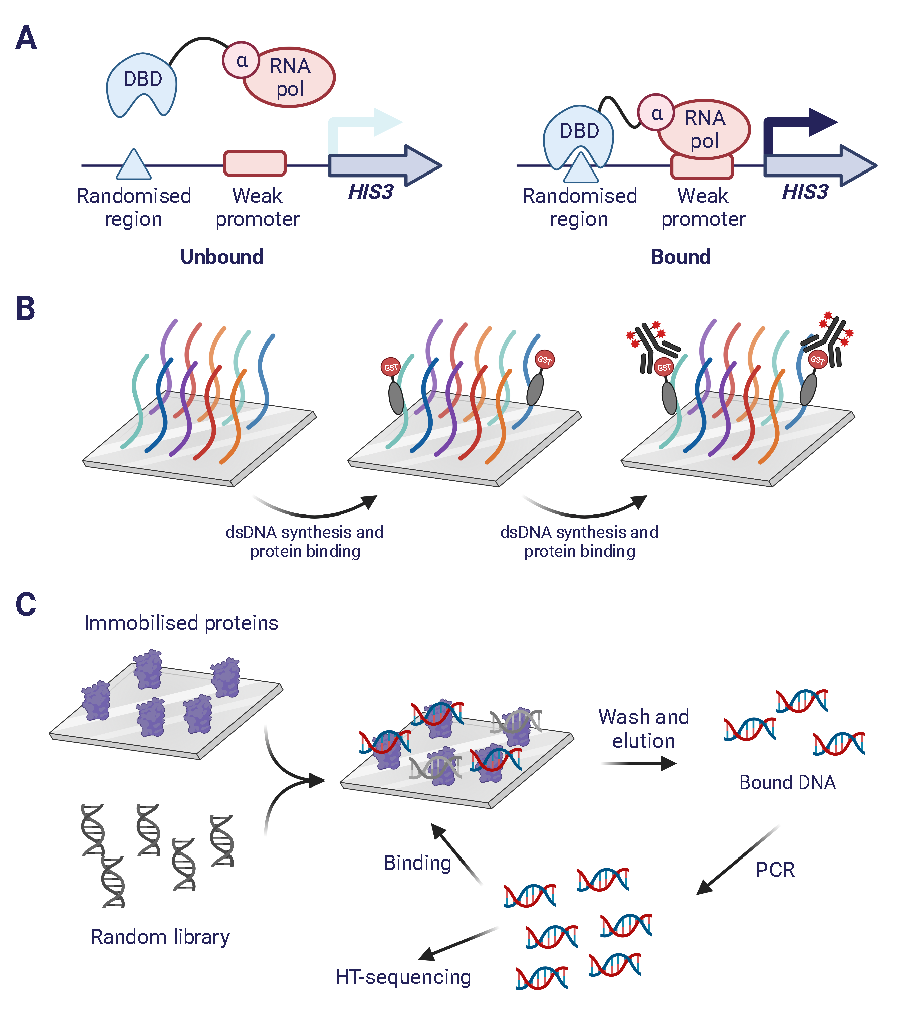
\includegraphics[width=0.9\textwidth]{chapter1/figures/fig7.pdf}
    \caption[Schematic views of three commonly-used high-throughput methods to study protein-DNA interactions \textit{in vitro}]{\textbf{Schematic views of three commonly-used high-throughput methods to study protein-DNA interactions \textit{in vitro}: B1H (A), PBM (B), and HT-SELEX (C).} See the main text for detailed descriptions (adapted from \cite{stormo2010determining}).}
    \label{fig:fig7}
\end{figure}

In the PBM, ssDNAs with common primers and spot-specific DNA sequences are immobilised on a microarray, and the ssDNAs are converted to dsDNA by extension using the common primer. The DBD of a transcription factor is fused to a tag (to date, only GST tag has been successfully used in the PBM) and purified. Then purified proteins are incubated with DNAs on the microarray, and the binding is visualised by incubating a fluorescence labelled antibody that recognises the tag (\textbf{Figure \ref{fig:fig7}B}). In this way, the binding of the transcription factor to all possible 10-mer sequences can be investigated.

HT-SELEX couples the traditional SELEX method with recent next generation sequencing technology. It utilises DNA ligands, each of which contains a 14-mer randomised DNA sequence, a 5-bp unique barcode and a universal sequencing primer for the high- throughput sequencing (usually an Illumina primer). The DNA ligands containing all possible 14-mer sequences are incubated with purified proteins immobilised to a 96-well plate. After washing off non-specific binding and elution, the bound DNA sequences are amplified and sequenced by high-throughput sequencing (\textbf{Figure \ref{fig:fig7}C}). HT-SELEX only requires a small amount of proteins (low nanogram levels), which is compatible with mammalian expression systems. Therefore, investigating the DNA binding of full-length proteins and proteins carrying post-translational modifications is possible.

\subsubsection{\textit{In vivo} methods}

\textit{In vitro} methods have generated valuable information, but \textit{in vitro} binding does not necessarily reflect \textit{in vivo} binding events. Fortunately, recent advances in chromatin immunoprecipitation (ChIP) followed by microarray (ChIP-chip) or by next generation sequencing (ChIP-seq) have enabled us to create a snapshot of the genome-wide binding profile of a specific transcription factor in a given cell type in a single experiment (reviewed in \cite{farnham2009insights}).

The first step of both ChIP-chip and ChIP-seq is the traditional ChIP assay: a protein of interest is covalently crosslinked to its DNA-binding sites or to another protein which directly contacts the DNA using crosslinkers, usually formaldehyde. After the shearing of the chromatin by sonication or enzymatic digestion, an antibody specific to the protein of interest is used to immunoprecipitate the protein-DNA adduct. After washing off the non- specific proteins bound by the antibody, the precipitated DNA fragments are reverse- crosslinked and purified. For ChIP-chip, the DNA samples are labelled with fluorescent dye and hybridised to designed microarrays (\textbf{Figure \ref{fig:fig8}}). For ChIP-seq, the sample is used to create a library that will be analysed by high-throughput next generation sequencing. The 5’ end of the DNA library is sequenced, and the resulting short sequencing reads, also known as tags (the terms reads and tags are interchangeable), are mapped back to a reference genome to identify the positions of the reads (\textbf{Figure \ref{fig:fig8}}). Then both methods require certain computational algorithms to detect the binding sites of the protein of interest (reviewed in \cite{park2009chip-seq:}).

\begin{figure}[h]
    \centering
    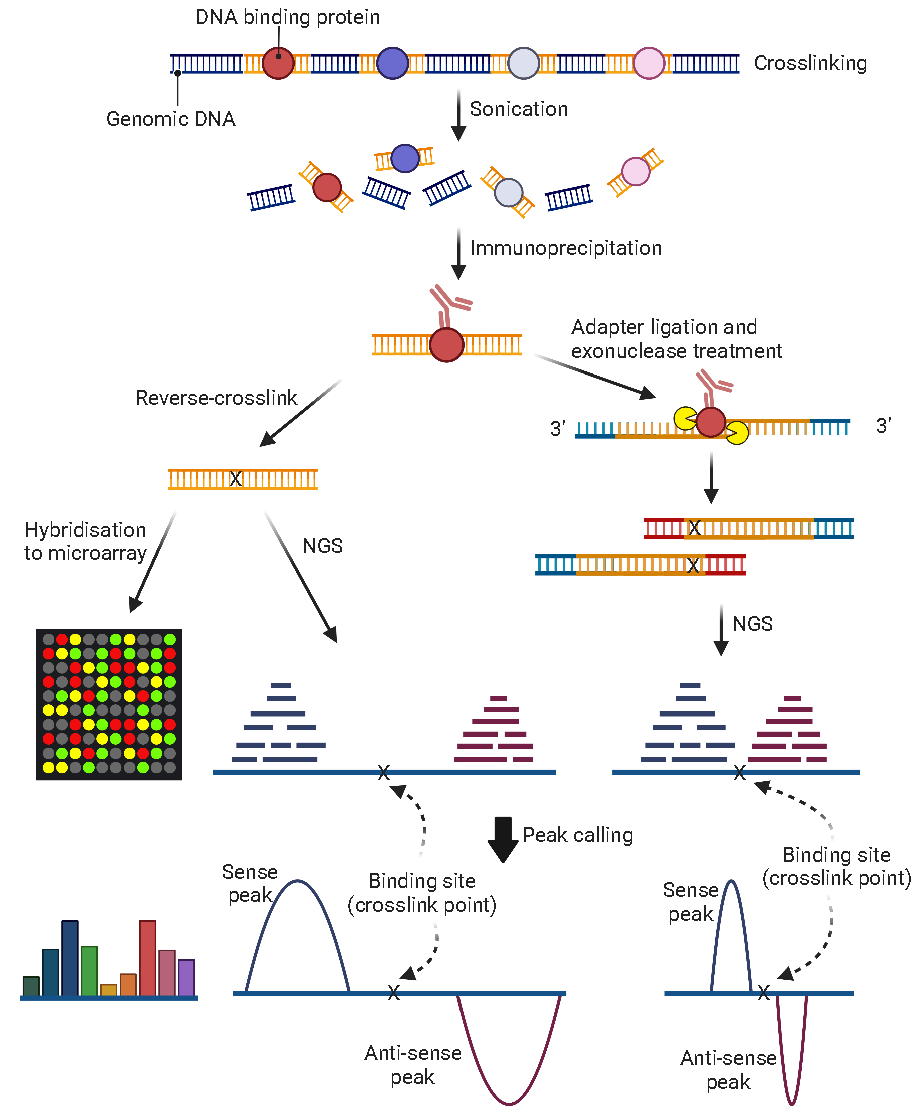
\includegraphics[width=0.8\textwidth]{chapter1/figures/fig8.pdf}
    \caption[Schematic views of the procedures of three ChIP-based technologies to study protein-DNA interactions \textit{in vivo}]{\textbf{Schematic views of the procedures of three ChIP-based technologies to study protein-DNA interactions \textit{in vivo.}} See detailed descriptions in the main text (adapted from \cite{visel2009genomic,rhee2011comprehensive}).}
    \label{fig:fig8}
\end{figure}

The quality of ChIP-chip results depend on the coverage, density and resolution of the microarray used for hybridisation (reviewed in \cite{hudson2006high-throughput}). The sequence covered in a single microarray is fairly limited compared to the large scale of the human genome, and the resolution as well as clarity of signal is often quite poor. As an alternative method, ChIP-seq offers many advantages over ChIP-chip, such as higher resolution and signal-to-noise ratio, and greater coverage (reviewed in \cite{park2009chip-seq:}). Hence, ChIP-seq is gradually replacing ChIP-chip. However, when investigating organisms with small genomes or a specific part of a large genome, ChIP-chip is still useful and more cost-effective.

Although ChIP-seq has higher resolution and signal-to-noise ratio than ChIP-chip, the binding events identified from ChIP-seq experiment are still too large to identify the exact binding sites of a protein due to the heterogeneous DNA fragments generated by the sonication. Another serious issue is that the contamination of non-crosslinked DNA in the ChIP samples, meaning the majority (60 - 90\%) of the sequencing readout is background (\cite{pepke2009computation,rhee2011comprehensive}). To improve the resolution and to reduce the background of ChIP-seq, a recent study applies an exonuclease to the ChIP sample before reverse-crosslinking, where the exonuclease trims the 5’ of the DNA to the exact crosslinking point (\textit{i.e.} the exact binding site) (\textbf{Figure \ref{fig:fig8}}). In addition, the non-crosslinked DNA will be degraded, and hence the background will be reduced. When proceeding to the sequencing step, the resulting short sequencing reads are just flanking the exact crosslinked site. This method, called ChIP-exo, significantly increases the resolution and reduces the background of ChIP-seq, and has been successfully used in both yeast and human cells, and for factors both directly and indirectly bind to DNA (\cite{rhee2011comprehensive,rhee2012genome-wide,yen2012genome-wide}).

All ChIP-based methods are exclusively dependent on high-quality antibodies which are not always available. Indeed, according to a recent assessment of the quality of histone modification antibodies, more than 20\% fail in ChIP (\cite{egelhofer2011an}). The available antibodies for transcription factors are much fewer than those for histone modifications. To circumvent the antibody issues, a method, called DamID, has been developed to identify the \textit{in vivo} protein-DNA interaction (\cite{van-steensel2000identification}). In the DamID, the protein of interest is fused to the bacterial Dam methyltransferase. When the protein binds to DNA, it also brings the Dam methyltransferase close to DNA where it can methylate the adenine of the GATC sequence nearby. Instead of using specific antibodies, one can identify the binding events by finding out the G\sus{m}ATC sequences which does not exist in the eukaryotic genome without introducing the Dam methyltransferase (\cite{van-steensel2000identification}). However, the resolution of this method depends on the frequency of the GATC tetramer site in the genome, and it cannot detect the dynamic binding between protein and DNA, \textit{i.e.} when the protein dissociates from the DNA, the methylated adenine will still be present. Therefore, the ChIP-based methods are still the golden standard for the study of \textit{in vivo} protein-DNA interactions.


\subsubsection{DNA binding by Forkhead transcription factors}

Early low-throughput \textit{in vitro} experiments, using selection of binding sites from pools of short random-sequence duplexes (\cite{pierrou1995selection}), revealed a seven-nucleotide core sequence as the Forkhead transcription factors binding sites. This consensus core that is recognised by the Forkhead domain is RYMAAYA, where R represents an A or G, Y represents a C or T, and M represents an A or C (\cite{kaufmann1995dna,overdier1994the,pierrou1994cloning}). Detailed comparison among the binding sites of FOXF2, FOXC1, FOXD1 and FOXL1 indicates that sequences both within and flanking the Forkhead consensus further determine the binding specificity of individual Forkhead transcription factors. Within the RYMAAYA core consensus, the heptameric sequence GTAAACA is the highest affinity site in most cases, except that FOXL1 prefers ATAAACA, and FOXC1 prefers GTAAATA (\cite{pierrou1994cloning}). At the flanking bases, the sequence preference of individual FOX proteins is relatively more variable than that within the core consensus. The flanking sequences also seem to be very important in the DNA-binding events of FOX proteins, because changes of the flanking sequences lead to different binding affinities for FOX proteins, or even failure to bind FOX proteins in spite of the presence of the core consensus (\cite{pierrou1994cloning}). Another study which compares the binding sites of FOXA, FOXQ1 and FOXD3 also confirms the observation that sequences within and flanking the core consensus determine the binding specificity of different Forkhead transcription factors (\cite{overdier1994the}). This is not a new discovery, because similar situations also exist in other proteins, such as the homeobox proteins and ETS-domain proteins, where specificity appears to be governed by nucleotides flanking their core consensus (\cite{ekker1991optimal,ekker1992differential,catron1993nucleotides,szymczyna2000dna}).

The third $\alpha$-helix $\alpha 3$ is the main DNA contact interface of Forkhead transcription factors, and the amino acids within this region are extremely conserved (reviewed in \cite{hannenhalli2009the}). Some Forkhead transcription factors (\textit{e.g.} FOXA3 and FOXD3) possess an almost identical recognition helix $\alpha 3$ and even use a similar mechanism for DNA recognition (reviewed in \cite{obsil2008structure/function}), but they still possess different DNA sequence preferences (\cite{overdier1994the}). It has been shown that these differences arise from less conserved regions outside of the main DNA-binding interface. The use of domain-swap chimeric proteins suggests that amino acids around the N-terminal border of helix $\alpha 3$ and in the wing W2 of the FOX domain determine, at least in part, the specificity (\cite{pierrou1994cloning}). Consistent with this discovery, another study used a series of HFH/HNF-3 protein chimeras and uncovered a 20-amino-acid region, which resides adjacent to the recognition helix $\alpha 3$, as responsible for determining their DNA-binding specificity (\cite{overdier1994the}). It is worth mentioning that a similar situation was also observed in ETS-domain proteins, where amino acid residues located away from the DNA- binding interface are found to be critical determinants for the binding specificity of individual ETS transcription factors (\cite{shore1996determinants}).

Recent high-throughput \textit{in vitro} experiments are consistent with previous findings. The DNA binding of mouse Forkhead transcription factors FOXA2, FOXJ1, FOXJ3, FOXK1 and FOXL1 have been analysed by PBM, and human FOXJ3 has been analysed by HT-SELEX. The core consensus RYMAAYA is the most frequent bound sequence, with GTAAACA being the highest affinity site in all cases. However, no apparent sequence preference for individual factor is observed (\cite{badis2009diversity,jolma2010multiplexed}).

Several human Forkhead transcription factors like FOXA (\cite{hurtado2011foxa1,motallebipour2009differential}), FOXH (\cite{kim2011chromatin}), FOXK (\cite{grant2012live-cell,ji2012the}) and FOXP (\cite{gabut2011an,katoh2011foxp3}) have been studied only recently by the ChIP-seq analyses. Motif searches reveal that responsive elements that resemble the Forkhead core consensus are enriched in the cistromes of all those factors. However, due to the differences of cell lines and computational algorithms used in different labs, it is difficult to explore the binding specificity of those Forkhead proteins. On the other hand, all of these studies have mainly focused on finding potential target genes and functions of individual Forkhead transcription factor, and none of these highlights the binding specificity of them.

Therefore, to explore the in vivo DNA binding specificity of individual Forkhead transcription factor, and more importantly to investigate the developmental and biological consequences of the binding specificity, it is better to perform ChIP-seq experiments of different members in the same cell line, and use the same computational approach to compare their DNA binding events.

\pagebreak

\section{Aims of the PhD project}

The healthy development of a living cell requires precise spatial-temporal gene expression. The first step of gene expression is transcription, which plays a central part in controlling the spatial-temporal gene expression. The general goal of studying transcription is to get an overall picture of how the whole transcriptional network controls gene expression, where transcription factors binding to DNA is a crucial step. To achieve this goal, one of the daunting challenges that we have to face is to understand the mechanisms of binding specificity of transcription factors. The overall aim of the project was to further our understanding of how transcription factors specifically recognise their target sites in the genome, when multiple family members can potentially converge on DNA sites with very similar sequences. Moreover, this then impacts on our ability to understand how a specific gene expression pattern can be generated in response to specific signals through a particular transcription factor. As a model system, we studied Forkhead transcription factors and in particular, the subgroup that impact on the cell cycle, especially on the G2 and M phases -- FOXK2, FOXM1 and FOXO3 transcription factors, all of which are ubiquitously expressed across a wide range of tissues and have their own specific functions. We chose to study their genome-wide binding events in the human osteosarcoma cell line U2OS, because it is a well-defined model cell line for the study of regulation of the cell cycle. Key questions that needed to be investigated include:

\begin{itemize}
    \item where do FOXK2, FOXM1 and FOXO3 bind in the genome?
    \item how are their DNA-binding specificities achieved?
    \item how is the binding specificity influenced by signalling pathways?
    \item how is the binding specificity related to their subsequent biological functions?
\end{itemize}